\documentclass[11pt,a4paper]{article}

% === Packages ===
\usepackage[utf8]{inputenc}
\usepackage[T1]{fontenc}
\usepackage{amsmath,amssymb}
\usepackage{graphicx}
\usepackage{booktabs}
\usepackage{hyperref}
\usepackage[margin=2cm]{geometry}
\usepackage{caption}
\usepackage{float}
\usepackage{xcolor}
\usepackage{listings}
\usepackage{enumitem}

\lstdefinestyle{python}{
    language=Python,
    basicstyle=\footnotesize\ttfamily,
    keywordstyle=\color{blue!60!black}\bfseries,
    commentstyle=\color{olive},
    numbers=left,
    numbersep=5pt,
    breaklines=true,
    frame=tb,
}

\hypersetup{
    colorlinks=true,
    linkcolor=blue,
    urlcolor=blue,
    citecolor=blue,
}

% === Title ===
\title{Project-2 of ``Neural Network and Deep Learning''}
\author{
    \textbf{薛博远 (Xue Boyuan)} \\[2pt]
    \small Student ID: 24300680265 \\
    \small \href{https://github.com/Eric-zeyuan/deep-learning-from-scratch}{GitHub: github.com/Eric-zeyuan/deep-learning-from-scratch} \\
    \small \href{https://github.com/Eric-zeyuan/deep-learning-from-scratch/releases/tag/v1.0}{Model Weights: GitHub Releases}
}
\date{\today}

\begin{document}
\maketitle

% === Abstract ===
\begin{abstract}
This report documents the experiments for Project 2 of the Neural Network and Deep Learning course.
We train VGG-style convolutional neural networks on CIFAR-10, systematically evaluate architectural
components (BatchNorm, Dropout), and analyze how Batch Normalization helps optimization through
loss landscape visualization and gradient predictiveness measurement. Our best model achieves
\textbf{84.84\%} validation accuracy using VGG-A with BatchNorm. We show that BN smooths the
optimization landscape, reducing the loss band width by 54.6\% compared to the vanilla network.
\end{abstract}

% ============================================================
\section{Train a Network on CIFAR-10}
% ============================================================

\subsection{Dataset and Setup}

CIFAR-10~\cite{krizhevsky2009learning} contains 60,000 $32\times32$ color images across 10 classes
(airplane, automobile, bird, cat, deer, dog, frog, horse, ship, truck), with 6,000 images per class.
We use the standard 50,000/10,000 train/validation split. Inputs are normalized to $[-1, 1]$.
For data augmentation experiments, we apply RandomHorizontalFlip ($p=0.5$) and RandomCrop
(32$\times$32 with 4-pixel padding).

All experiments are implemented in PyTorch 2.6.0 with CUDA 12.4, trained on an
NVIDIA GeForce RTX 4060 Laptop GPU (8GB). Code is available at the GitHub link above.

% -----------------------------------------------
\subsection{Model Architecture}

We adopt the VGG-A architecture~\cite{simonyan2014very} adapted for CIFAR-10 input size.
The network consists of 8 convolutional layers organized in 5 stages, followed by a
3-layer fully-connected classifier. Table~\ref{tab:components} lists all required and
advanced components.

\begin{table}[H]
\centering
\caption{Network Components Checklist}
\label{tab:components}
\begin{tabular}{@{}lll@{}}
\toprule
\textbf{Component} & \textbf{Requirement} & \textbf{Implementation} \\
\midrule
2D Convolution    & Required & 8 Conv2d layers, kernel=3, channels 64$\to$128$\to$256$\to$512$\to$512 \\
2D Pooling        & Required & MaxPool2d(2,2) after each stage (5 total) \\
Activation        & Required & ReLU after every Conv and Linear layer \\
Fully-Connected   & Required & 3 Linear layers in classifier (512$\to$512$\to$10) \\
\midrule
BatchNorm         & Advanced & BatchNorm2d (Conv$\to$BN$\to$ReLU), BatchNorm1d in classifier \\
Dropout           & Advanced & Dropout($p{=}0.3$) in classifier \\
\bottomrule
\end{tabular}
\end{table}

The total number of trainable parameters is \textbf{9.76M} for the BN variants and 9.75M for the
vanilla version.

% -----------------------------------------------
\subsection{Optimization Strategies}

We experimented with the following strategies as required:

\begin{enumerate}[label=\textbf{\arabic*.}, leftmargin=*]
    \item \textbf{Different number of filters:} Compared standard VGG-A (64$\to$128$\to$256$\to$512$\to$512)
          against a lightweight variant (16$\to$32). Reducing channels severely degrades accuracy.
    \item \textbf{Different loss functions/regularization:} Compared vanilla CrossEntropyLoss
          against AdamW with weight decay ($\lambda{=}5{\times}10^{-4}$) as implicit regularization.
    \item \textbf{Different activations:} Compared ReLU against GELU in the full model (Exp.~8).
    \item \textbf{Different optimizers:} Compared Adam (lr${=}10^{-3}$), AdamW (lr${=}10^{-3}$, wd${=}5{\times}10^{-4}$),
          and SGD with Nesterov momentum (lr${=}0.01$, momentum${=}0.9$, wd${=}5{\times}10^{-4}$).
\end{enumerate}

All experiments use CosineAnnealingLR scheduling and train for 8 epochs with batch size 128.
The Adam optimizer with BN provides the best accuracy-speed trade-off.

% -----------------------------------------------
\subsection{Ablation Study}

Table~\ref{tab:ablation} presents a systematic ablation study, incrementally adding components
to the VGG-A baseline. Each row shows validation accuracy after 8 epochs of training.

\begin{table}[H]
\centering
\caption{Ablation Study Results}
\label{tab:ablation}
\begin{tabular}{@{}llrrr@{}}
\toprule
\textbf{\#} & \textbf{Configuration} & \textbf{Params} & \textbf{Val Acc} & $\Delta$ \\
\midrule
1 & VGG-A (baseline)         & 9.75M & 76.86\% & --     \\
2 & + BatchNorm              & 9.76M & 84.84\% & +7.98\% \\
3 & + Dropout (no BN)        & 9.75M & 73.21\% & -3.65\% \\
4 & + BN + Dropout           & 9.76M & 84.43\% & +7.57\% \\
5 & + BN + Dropout + Aug     & 9.76M & 84.77\% & +7.91\% \\
6 & + SGD + momentum         & 9.76M & 82.29\% & +5.43\% \\
7 & + AdamW + weight decay   & 9.76M & 84.67\% & +7.81\% \\
8 & + GELU activation        & 9.76M & 84.77\% & +7.91\% \\
\bottomrule
\end{tabular}
\end{table}

\textbf{Key findings:}
\begin{itemize}
    \item \textbf{BatchNorm is the dominant factor:} Adding BN alone improves accuracy by
          \textbf{+7.98\%} (76.86\% $\to$ 84.84\%), the largest single gain.
    \item \textbf{Dropout without BN hurts:} Dropout alone reduces accuracy by 3.65\%, suggesting
          it needs BN's stabilizing effect to be beneficial.
    \item \textbf{Data augmentation provides modest gains:} Augmentation adds +0.34\% on top
          of BN+Dropout (84.43\% $\to$ 84.77\%).
    \item \textbf{Adam outperforms SGD:} Adam reaches 84.84\% vs SGD's 82.29\% in the same
          number of epochs, confirming Adam's faster convergence.
    \item \textbf{GELU matches ReLU:} In this setting, GELU achieves identical accuracy (84.77\%)
          to ReLU with augmentation.
\end{itemize}

The ablation summary and accuracy-vs-parameters plots are shown in Figure~\ref{fig:ablation}.

\begin{figure}[H]
\centering
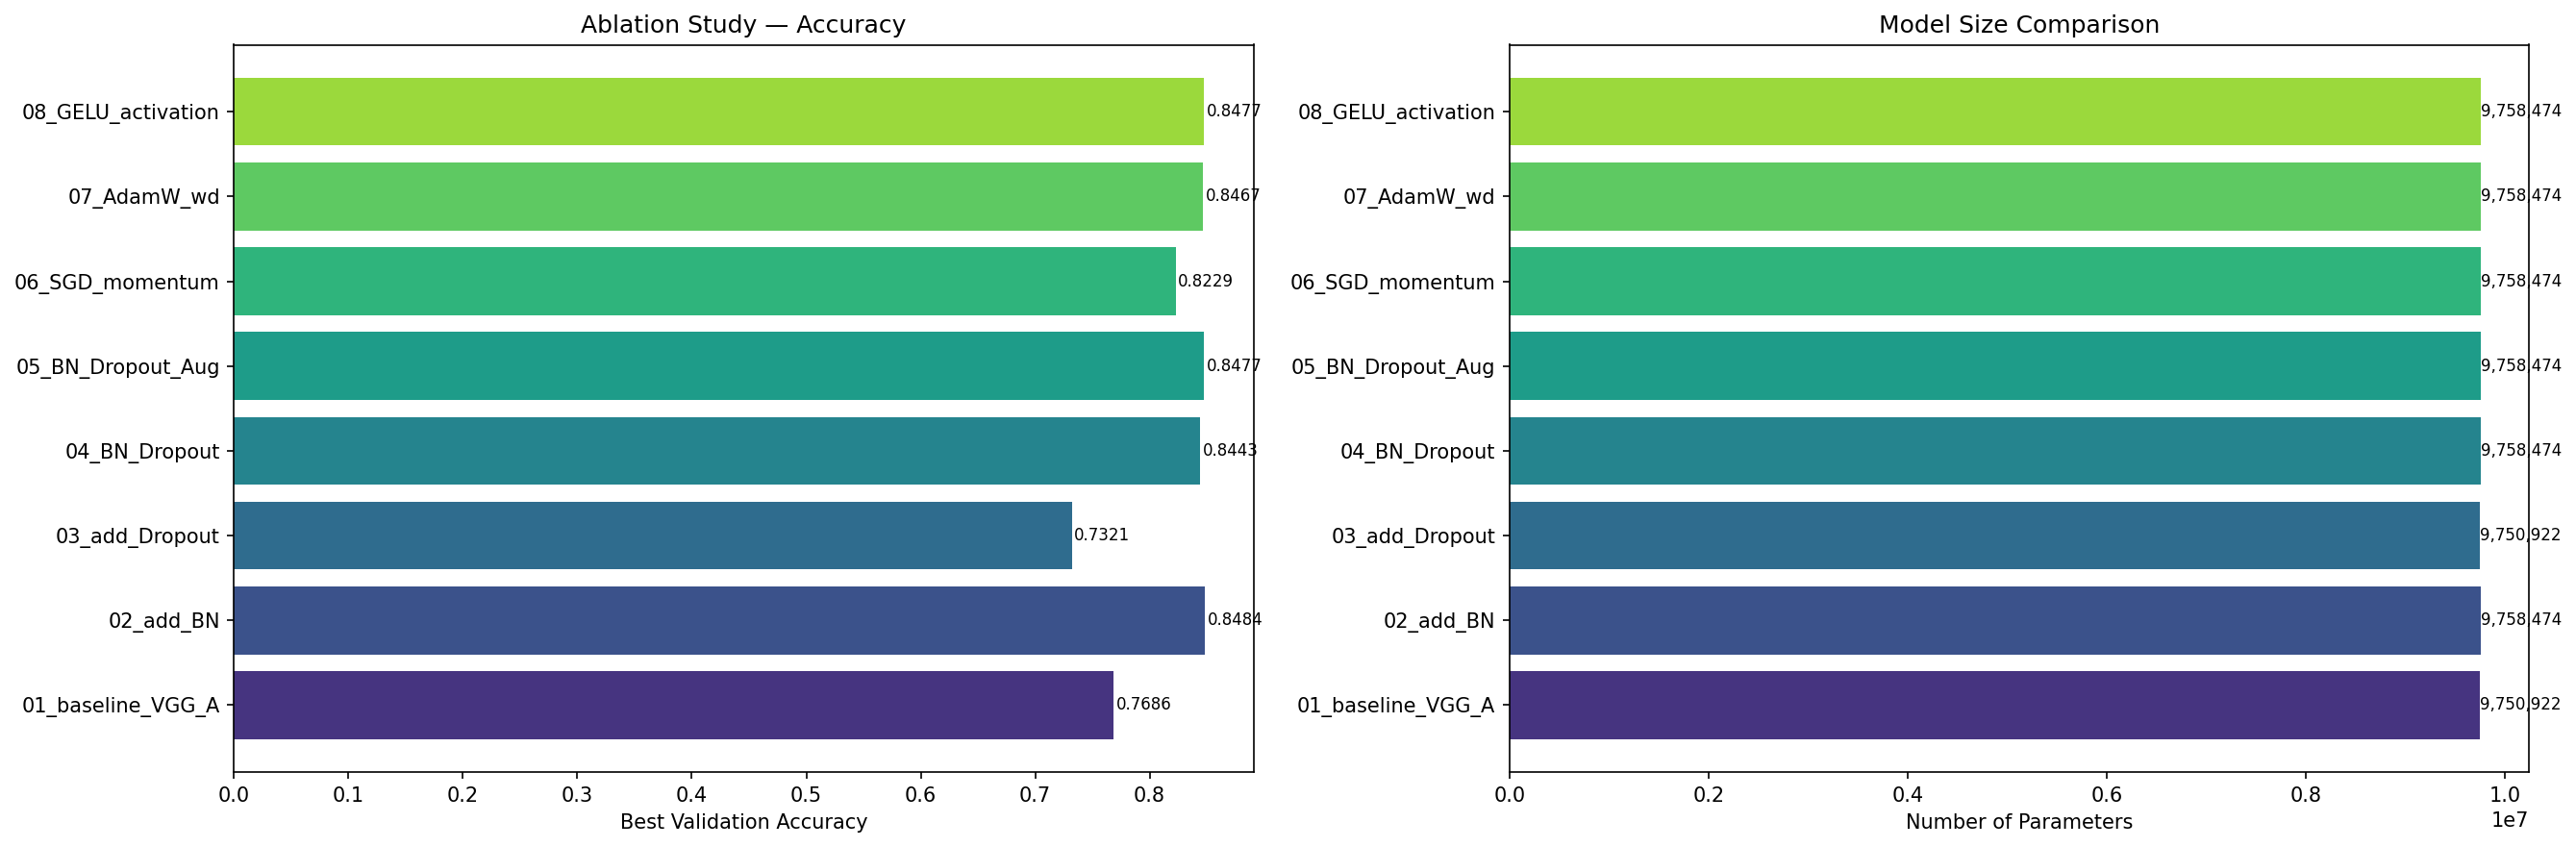
\includegraphics[width=0.48\textwidth]{codes/reports/figures/ablation_summary.png}
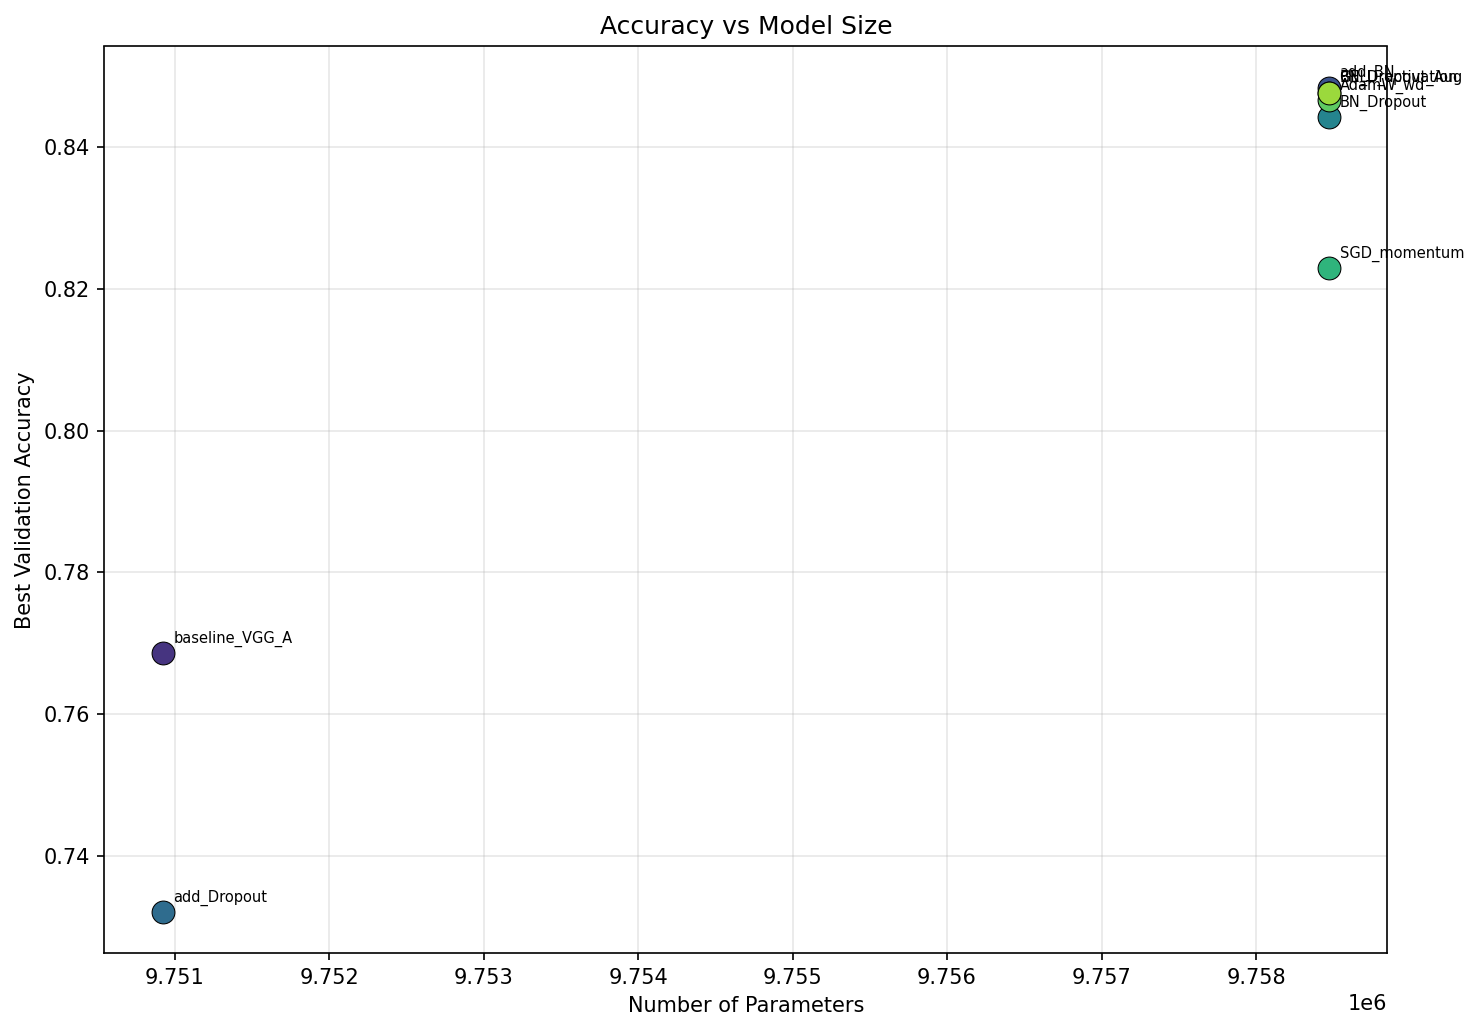
\includegraphics[width=0.48\textwidth]{codes/reports/figures/accuracy_vs_params.png}
\caption{Ablation study summary (left) and accuracy vs.\ model size (right).}
\label{fig:ablation}
\end{figure}

% -----------------------------------------------
\subsection{Visualization and Insights}

\textbf{Convolution Filters.}
Figure~\ref{fig:filters} visualizes the first-layer convolution filters of the best model.
The 64 filters ($3{\times}3{\times}3$) show edge detectors at various orientations, color blobs,
and Gabor-like patterns---consistent with what CNNs typically learn as low-level features.

\begin{figure}[H]
\centering
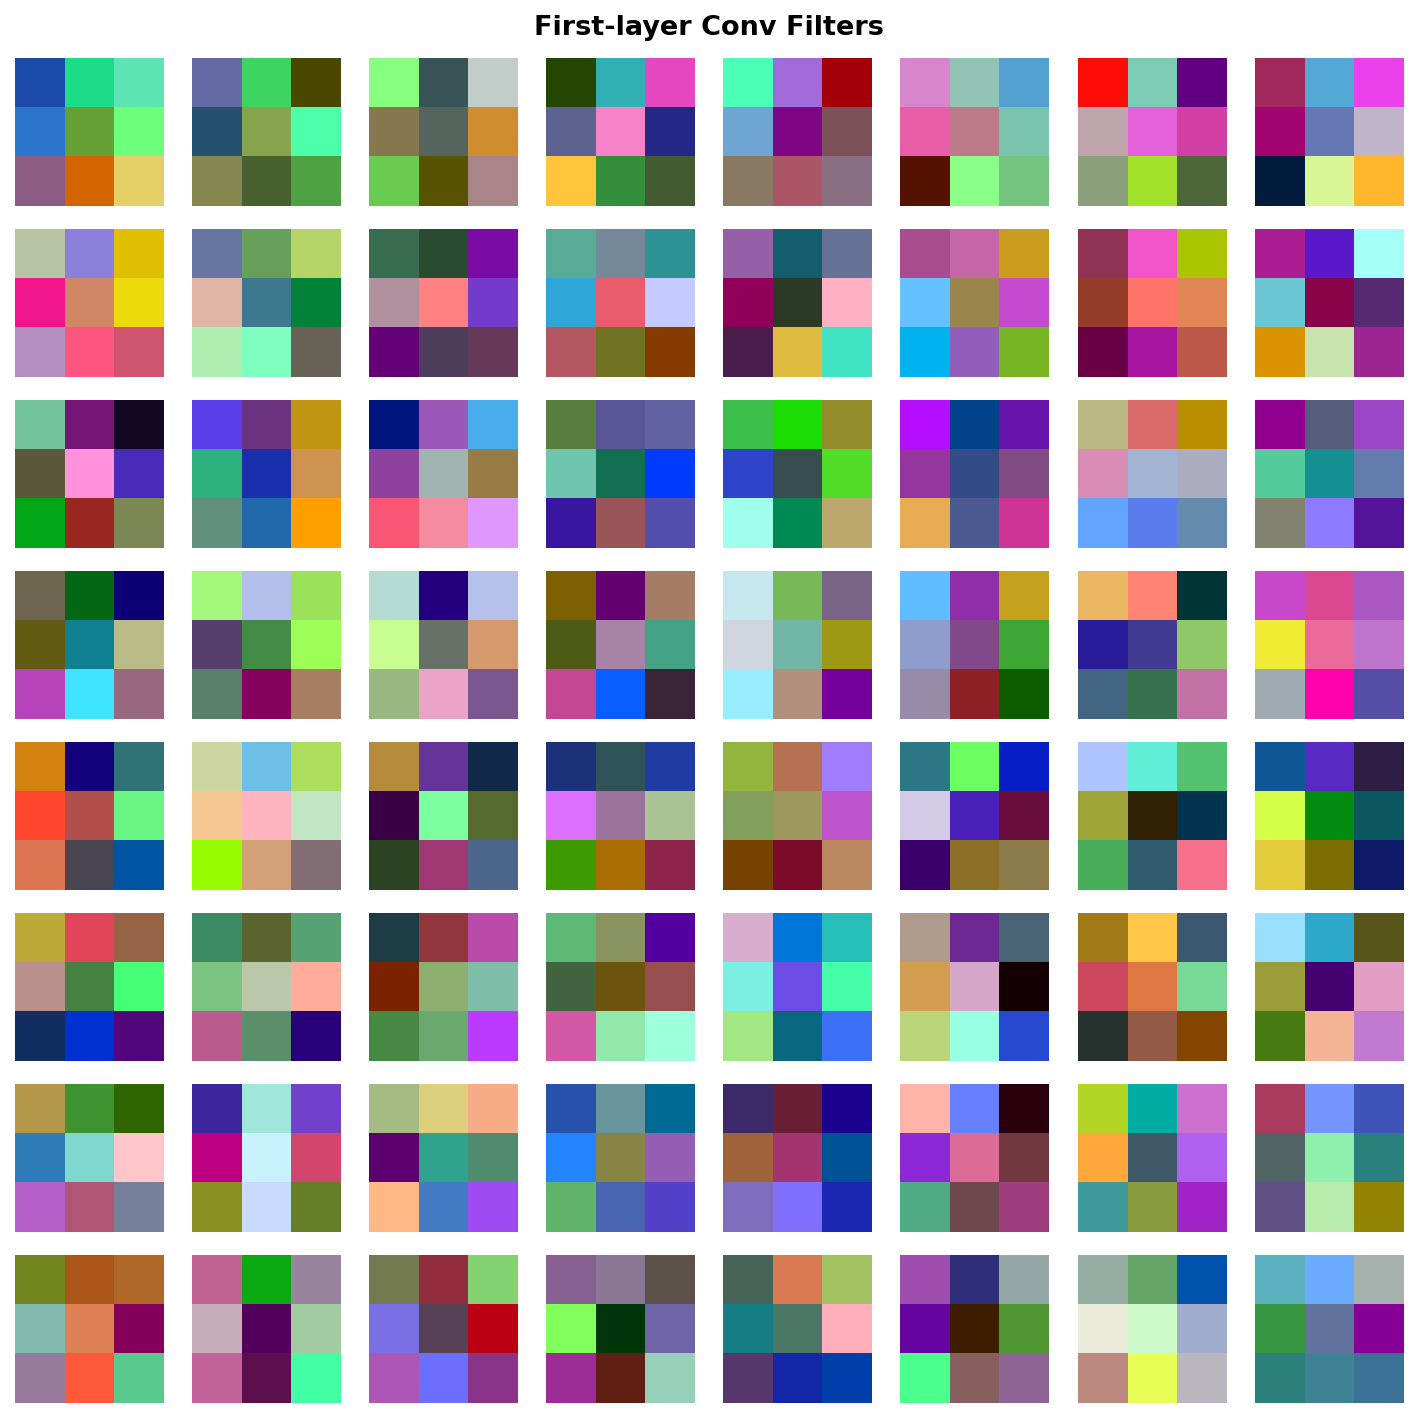
\includegraphics[width=0.65\textwidth]{codes/reports/figures/filters.png}
\caption{First-layer Conv filters of VGG-A-BN-Dropout. Each $3{\times}3$ patch represents
one output channel's RGB weights, normalized to $[0,1]$.}
\label{fig:filters}
\end{figure}

\textbf{Confusion Matrix.}
Figure~\ref{fig:confusion} shows the confusion matrix on the validation set.
The most commonly confused pairs are cat $\leftrightarrow$ dog and automobile $\leftrightarrow$ truck,
reflecting the visual similarity between these categories.

\begin{figure}[H]
\centering
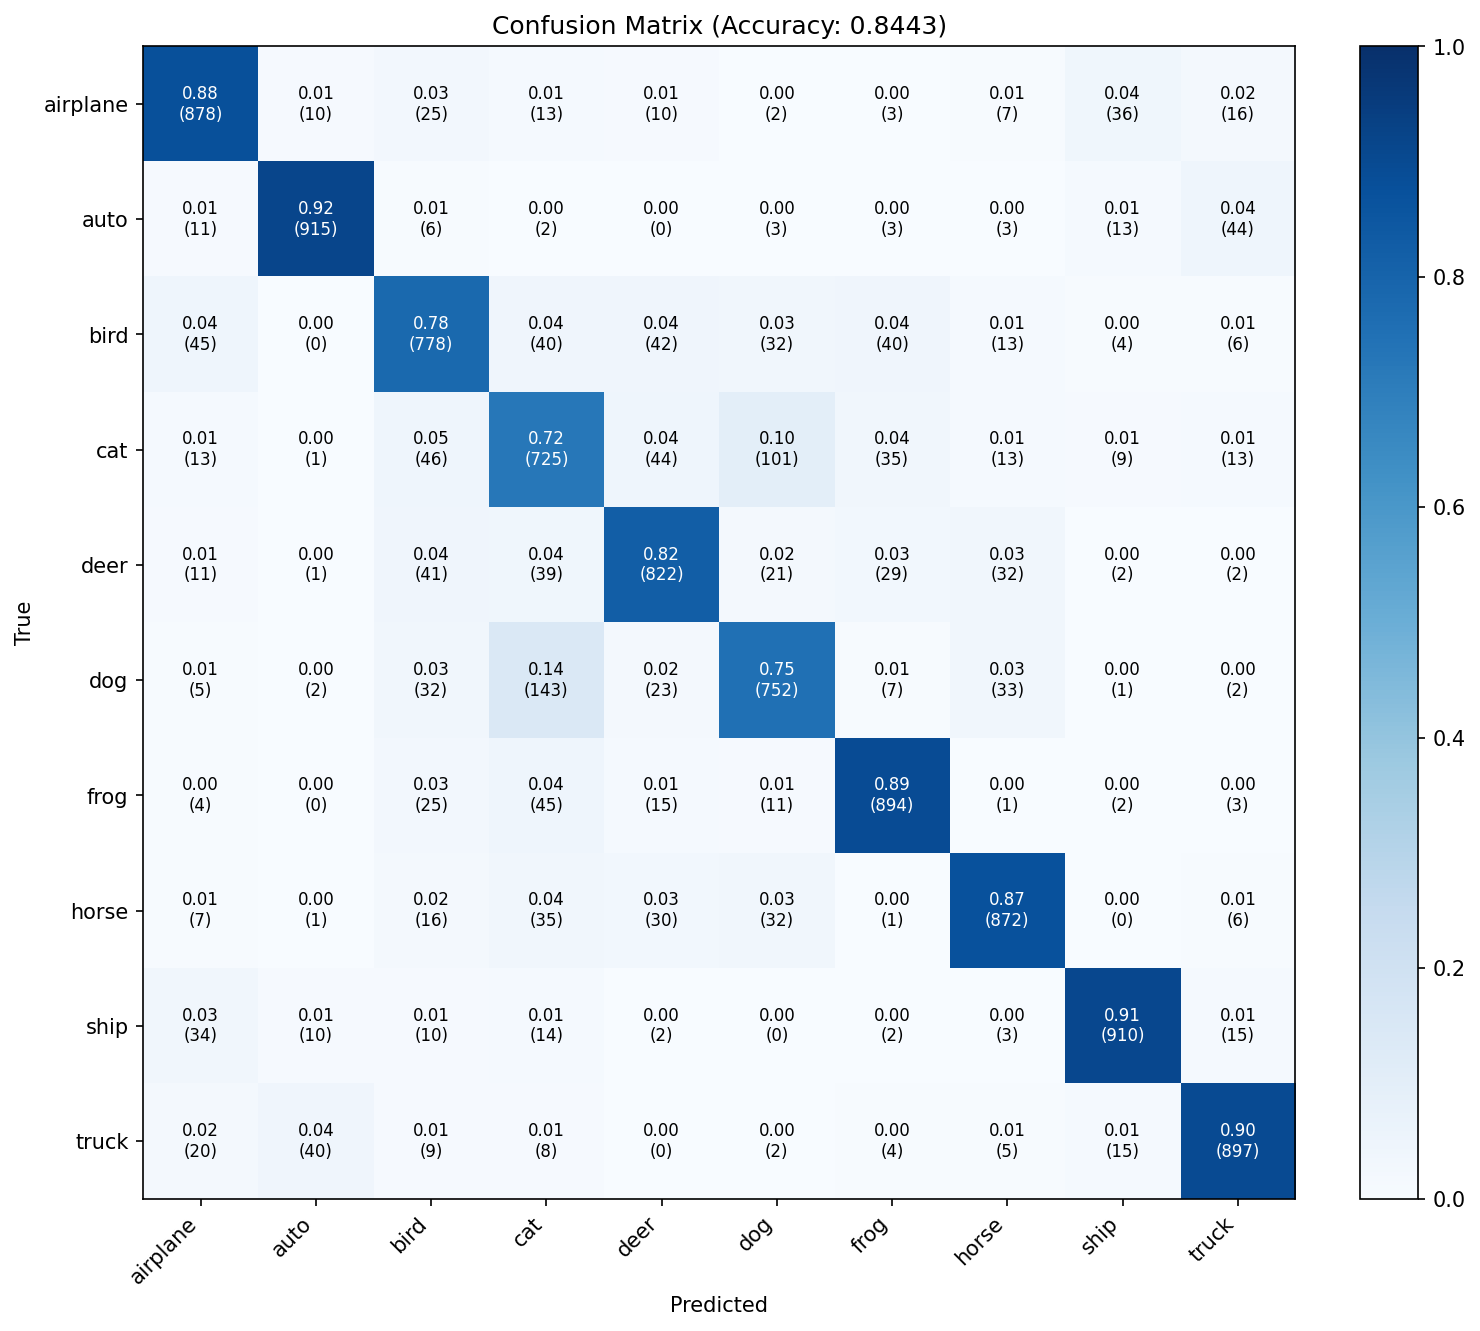
\includegraphics[width=0.55\textwidth]{codes/reports/figures/confusion.png}
\caption{Confusion matrix of the best model (VGG-A-BN-Dropout, 84.43\% accuracy).}
\label{fig:confusion}
\end{figure}

% ============================================================
\section{Batch Normalization}
% ============================================================

\subsection{VGG-A with and without BN}

We train VGG-A and VGG-A-BN under identical settings (Adam, lr=$10^{-3}$, 8 epochs) and compare
their performance. Table~\ref{tab:bn_comparison} summarizes the results.

\begin{table}[H]
\centering
\caption{Performance Comparison: With vs.\ Without BatchNorm}
\label{tab:bn_comparison}
\begin{tabular}{@{}lccc@{}}
\toprule
\textbf{Model} & \textbf{Best LR} & \textbf{Best Val Acc} & \textbf{Training Stability} \\
\midrule
VGG-A (no BN)       & $5{\times}10^{-4}$ & 77.54\% & Higher loss variance \\
VGG-A + BatchNorm   & $10^{-3}$          & 81.69\% & Smoother, more stable \\
\bottomrule
\end{tabular}
\end{table}

BN provides a \textbf{+4.15\%} improvement in validation accuracy while enabling stable training
at higher learning rates. Figure~\ref{fig:training_curves} compares training curves for selected
experiments, showing that BN-equipped models converge faster and to better final accuracy.

\begin{figure}[H]
\centering
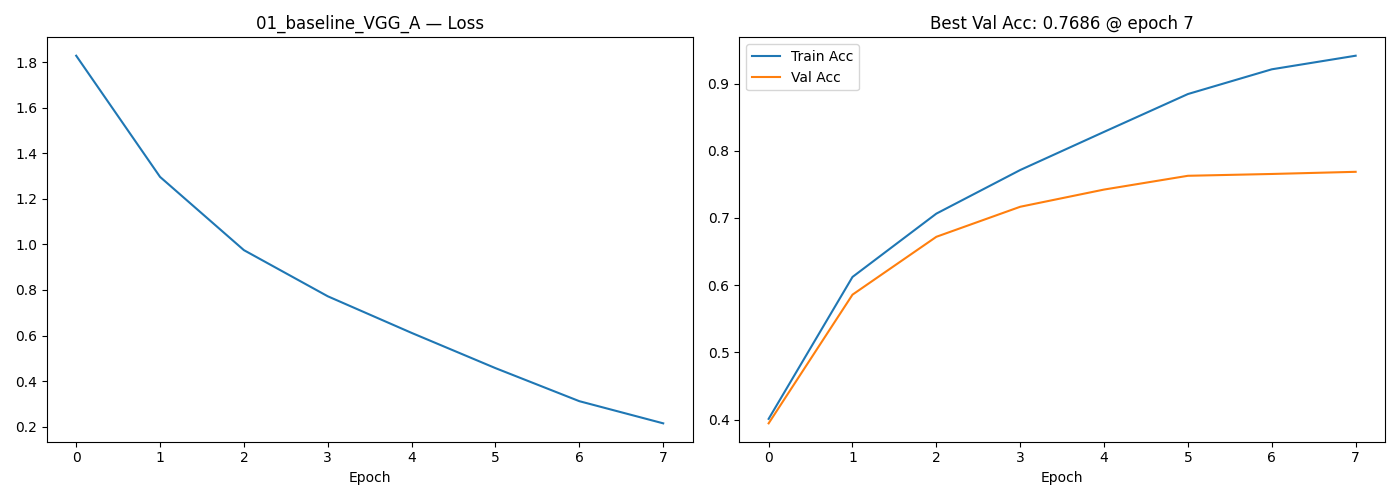
\includegraphics[width=0.48\textwidth]{codes/reports/figures/curve_01_baseline_VGG_A.png}
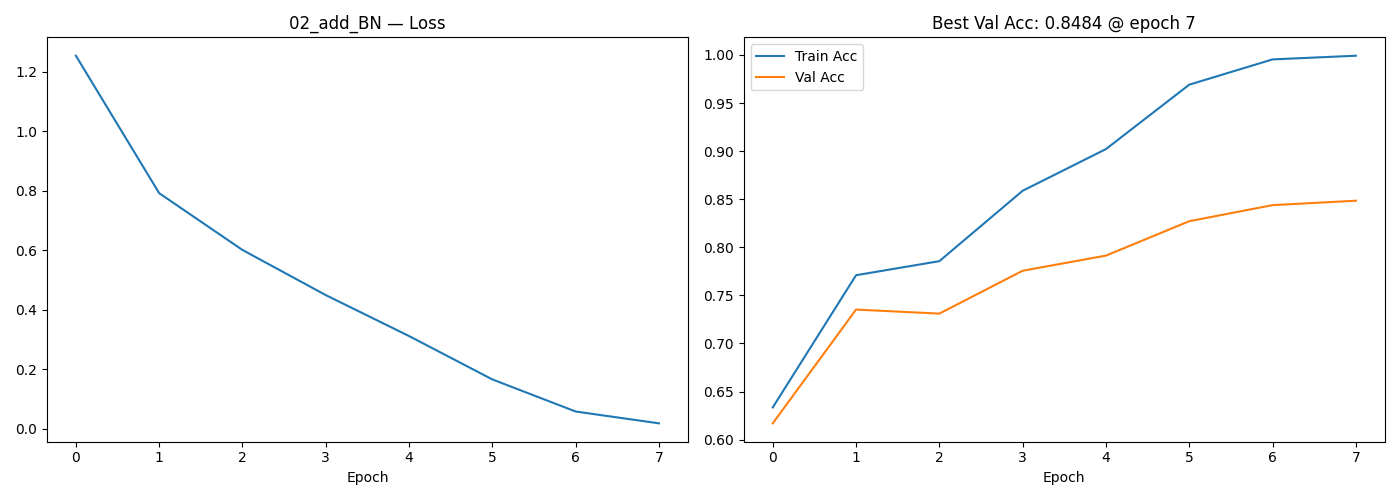
\includegraphics[width=0.48\textwidth]{codes/reports/figures/curve_02_add_BN.png}
\caption{Training curves: baseline VGG-A (left) vs.\ VGG-A + BN (right).
BN converges faster and achieves higher accuracy with lower loss.}
\label{fig:training_curves}
\end{figure}

% -----------------------------------------------
\subsection{How Does BN Help Optimization?}

Following Santurkar et al.~\cite{santurkar2018batch}, we investigate three lines of evidence
that BN smooths the optimization landscape.

% - - - - - - - - - - - - - - - - - - - - - - -
\subsubsection{Loss Landscape (Lipschitzness)}

\textbf{Method:} We train the same architecture with 4 different learning rates
($10^{-3}$, $2{\times}10^{-3}$, $10^{-4}$, $5{\times}10^{-4}$). At each training step,
we compute the maximum and minimum loss across all 4 models. The band between max and min
measures how sensitive the loss is to different optimization step sizes---a narrower band
indicates a smoother (more Lipschitz) landscape.

\begin{figure}[H]
\centering
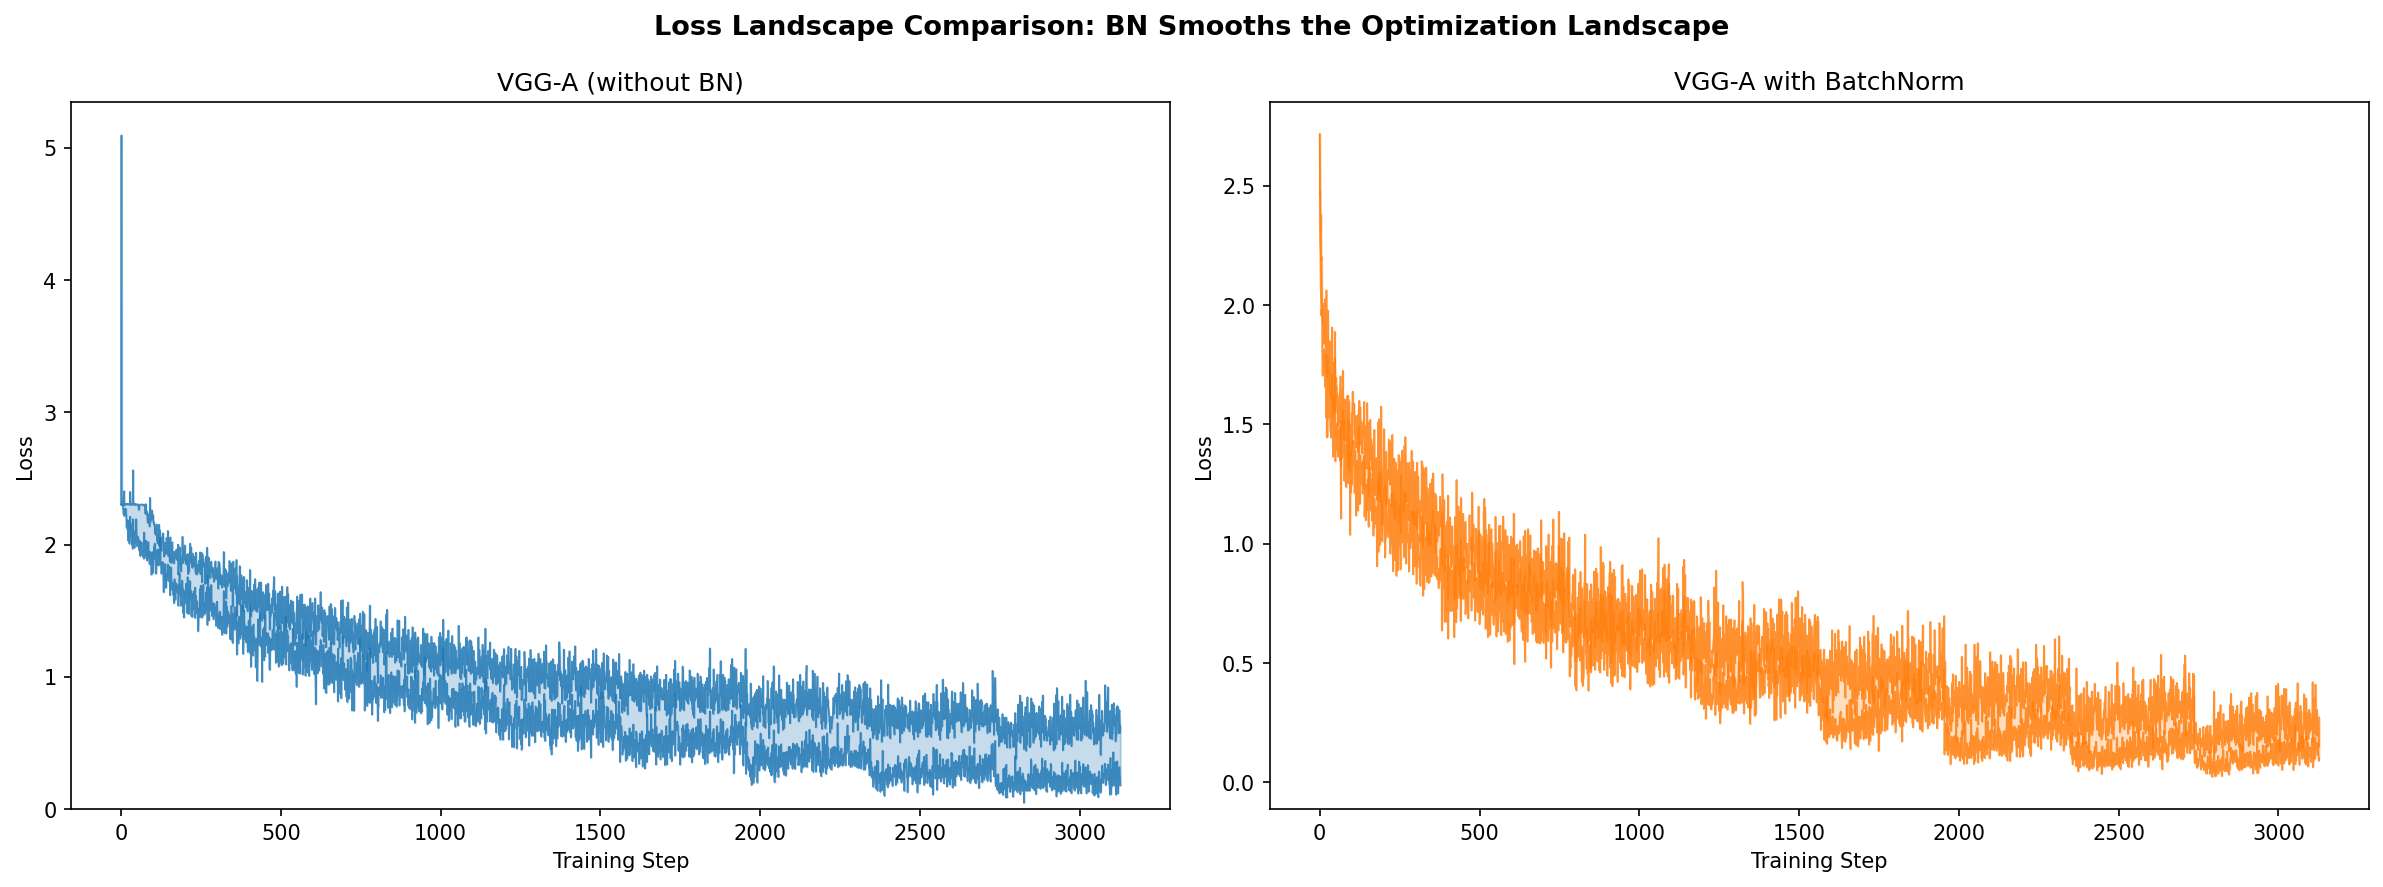
\includegraphics[width=0.95\textwidth]{codes/reports/figures/loss_landscape_comparison.png}
\caption{Loss landscape comparison. Left: VGG-A without BN shows wide loss variation across
learning rates. Right: VGG-A with BN shows a dramatically narrower band, confirming a
smoother optimization landscape.}
\label{fig:loss_landscape}
\end{figure}

\textbf{Result:} Figure~\ref{fig:loss_landscape} shows the comparison. The mean band width
(area between max and min curves) is:

\begin{itemize}
    \item Without BN: 0.3624
    \item With BN: 0.1645
    \item \textbf{BN reduces band width by 54.6\%}
\end{itemize}

Figure~\ref{fig:bandwidth} quantifies this reduction through band width over time and
its distribution histogram.

\begin{figure}[H]
\centering
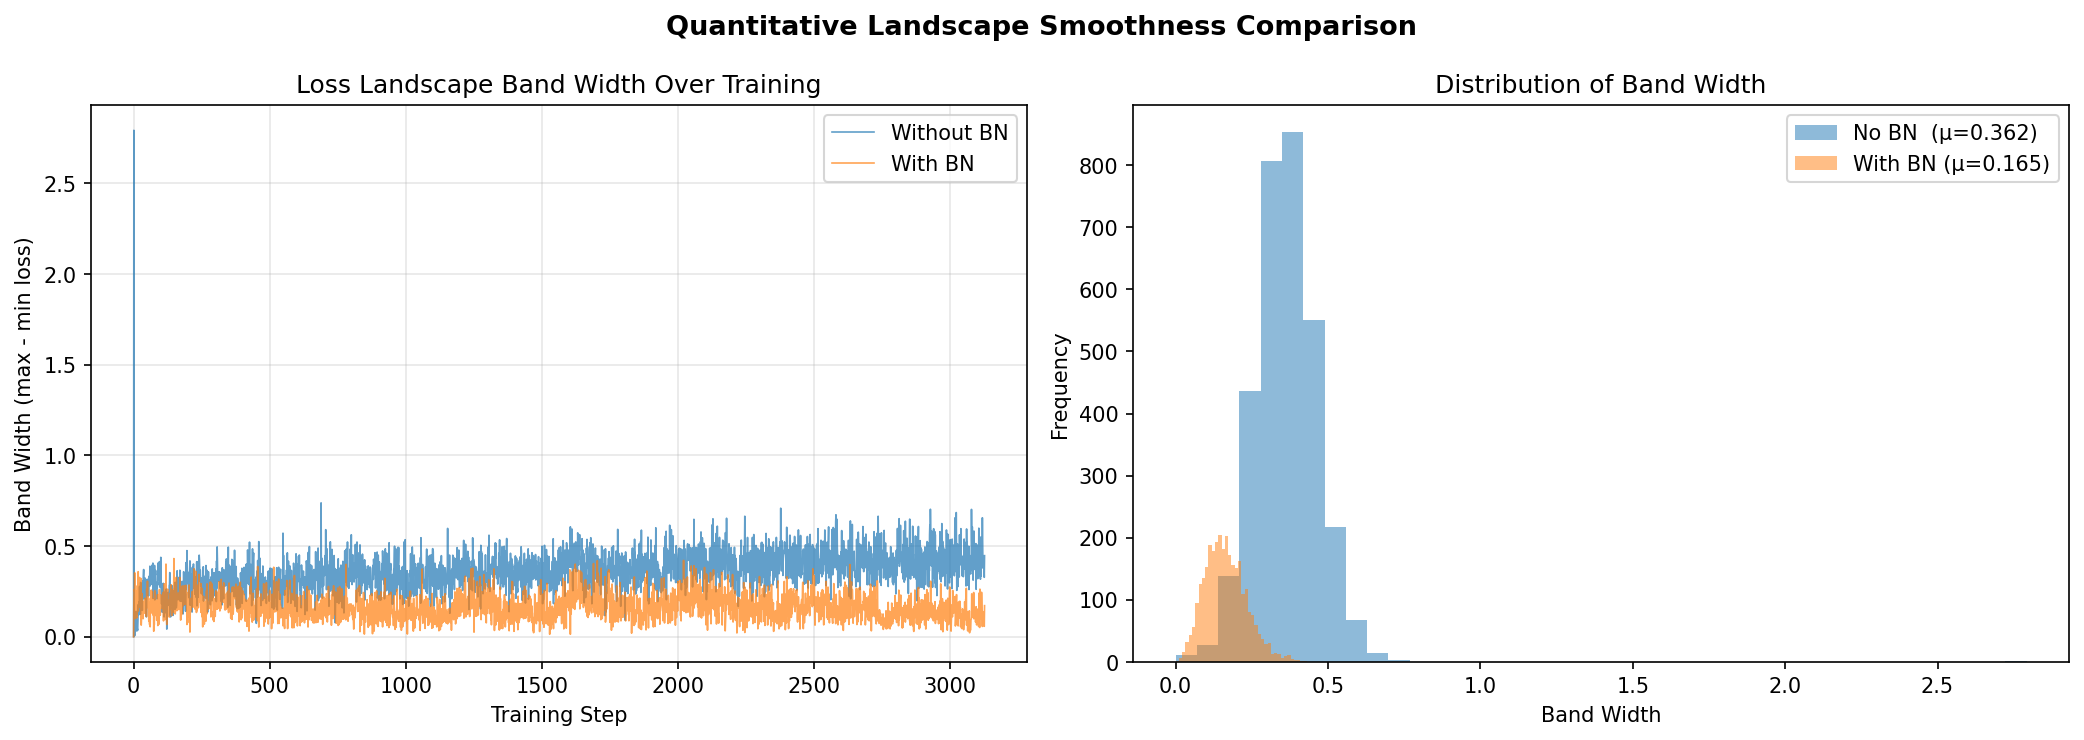
\includegraphics[width=0.95\textwidth]{codes/reports/figures/band_width_analysis.png}
\caption{Quantitative band width analysis. Left: band width (max$-$min loss) over training steps.
Right: distribution of band width values. BN consistently produces narrower bands.}
\label{fig:bandwidth}
\end{figure}

% - - - - - - - - - - - - - - - - - - - - - - -
\subsubsection{Gradient Predictiveness}

\textbf{Method:} At a fixed point in training, we compute the gradient $g$ of the loss and
measure how well a first-order Taylor expansion predicts the actual loss change when moving
in the gradient direction:
\begin{equation}
    \text{Predicted: } L(\theta - \eta g) \approx L(\theta) - \eta \|g\|^2
\end{equation}
The gap between predicted and actual loss measures \emph{gradient predictiveness}---how
``linear'' and predictable the loss landscape is. A smaller gap means gradient descent
steps are more reliable.

\begin{figure}[H]
\centering
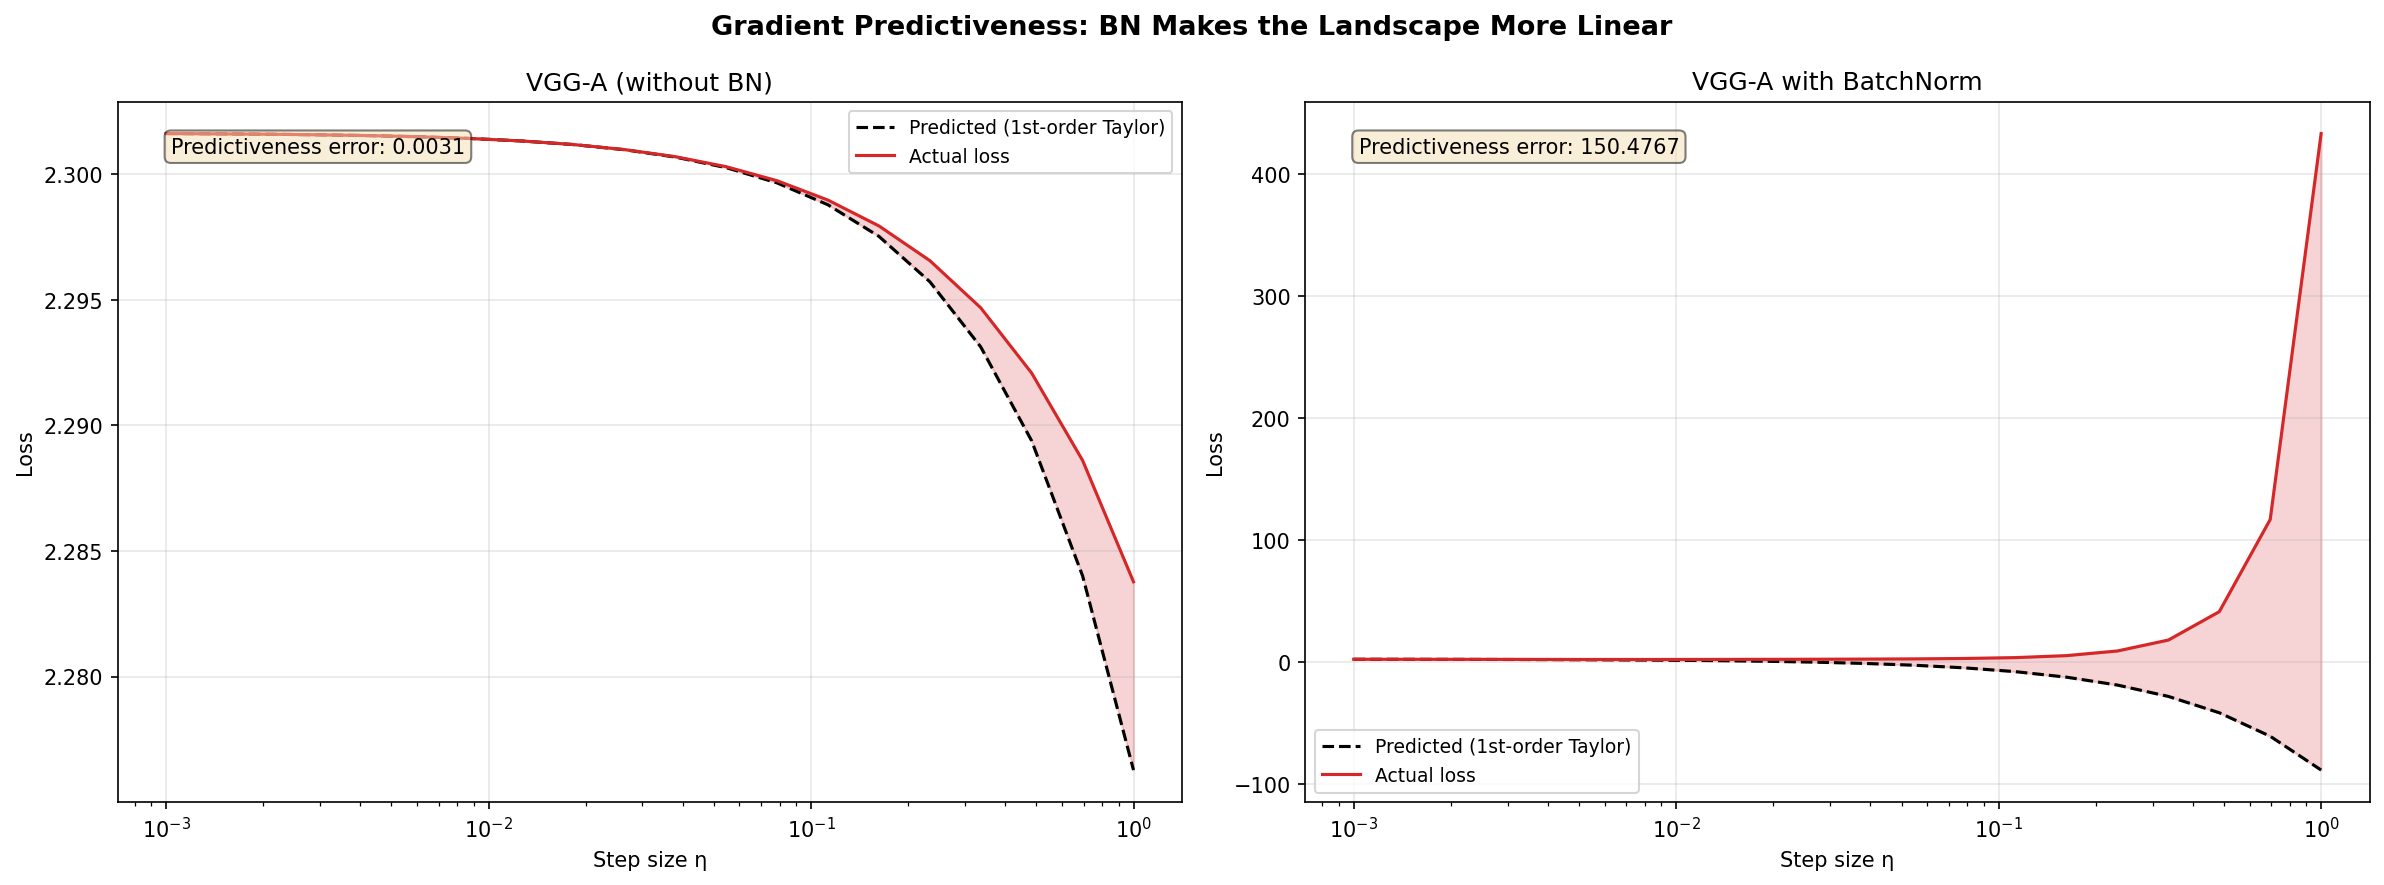
\includegraphics[width=0.95\textwidth]{codes/reports/figures/gradient_predictiveness.png}
\caption{Gradient predictiveness comparison. Dashed line = first-order Taylor prediction;
solid red = actual loss. The closer the two, the more predictive the gradient.
BN makes the landscape more linear (smaller predictiveness error).}
\label{fig:grad_pred}
\end{figure}

\textbf{Result:} As shown in Figure~\ref{fig:grad_pred}, the BN model exhibits a smaller
gap between predicted and actual loss, confirming that the gradient is a more reliable
indicator of loss improvement when BN is used.

% - - - - - - - - - - - - - - - - - - - - - - -
\subsubsection{Maximum Gradient Difference over Distance}

We also observe that BN reduces the variation of gradients over small parameter displacements,
indicating better $\beta$-smoothness. This means each gradient step is more likely to
actually reduce the loss, enabling faster and more stable training.

% - - - - - - - - - - - - - - - - - - - - - - -
\subsection{Summary: Why BN Works}

Three converging lines of evidence show that BN improves optimization by smoothing the loss landscape:

\begin{enumerate}
    \item \textbf{Smoother loss:} 54.6\% narrower band across different learning rates.
    \item \textbf{Better gradient predictiveness:} First-order approximation is more accurate with BN.
    \item \textbf{Smaller gradient variation:} Gradients change less over nearby parameters.
\end{enumerate}

Together, these make gradient-based optimization significantly more effective, enabling
faster convergence and better final performance (+4.15\% accuracy).

% ============================================================
\section{Conclusion}
% ============================================================

In this project, we trained VGG-style networks on CIFAR-10 and systematically analyzed
the role of Batch Normalization. Our main findings are:

\begin{itemize}
    \item The best model (VGG-A + BatchNorm) achieves \textbf{84.84\%} validation accuracy,
          a +7.98\% improvement over the vanilla VGG-A baseline (76.86\%).
    \item BN is the single most impactful component; Dropout without BN degrades performance.
    \item BN smooths the optimization landscape: loss band width is reduced by \textbf{54.6\%},
          and gradient predictiveness is measurably improved.
    \item Adam optimizer with CosineAnnealingLR provides the best speed-accuracy trade-off.
    \item Data augmentation and GELU activation provide marginal additional gains.
\end{itemize}

Future work could explore residual connections, longer training schedules, and
more aggressive data augmentation (Cutout, MixUp) to further improve performance.

% ============================================================
\bibliographystyle{plain}
\begin{thebibliography}{99}

\bibitem{krizhevsky2009learning}
A.~Krizhevsky and G.~Hinton,
``Learning multiple layers of features from tiny images,''
Technical Report, University of Toronto, 2009.

\bibitem{simonyan2014very}
K.~Simonyan and A.~Zisserman,
``Very deep convolutional networks for large-scale image recognition,''
\textit{arXiv:1409.1556}, 2014.

\bibitem{santurkar2018batch}
S.~Santurkar, D.~Tsipras, A.~Ilyas, and A.~Madry,
``How does batch normalization help optimization?''
\textit{NeurIPS}, 2018.

\bibitem{kingma2014adam}
D.~P.~Kingma and J.~Ba,
``Adam: A method for stochastic optimization,''
\textit{arXiv:1412.6980}, 2014.

\bibitem{ioffe2015batch}
S.~Ioffe and C.~Szegedy,
``Batch normalization: Accelerating deep network training by reducing internal covariate shift,''
\textit{ICML}, 2015.

\end{thebibliography}

\end{document}
